\documentclass[a4paper]{article}


\usepackage{alphabeta} 
\usepackage{enumitem} 
\usepackage{mathtools}
\usepackage{amsmath, amssymb} 
\usepackage{amsthm}
\usepackage{cancel} 
\usepackage[margin=0.70in]{geometry} 
\geometry{left=3cm,right=3cm,top=2.4cm,bottom=2.4cm}	%the page geometry as defined, A4=210x297mm
\usepackage{graphicx}
\usepackage{wrapfig}
\usepackage[center]{caption}
\usepackage{textcomp}
\usepackage{tabto}
\usepackage{layout}
\usepackage{bm}
\usepackage{minipage-marginpar}
\usepackage[dvipsnames]{xcolor}
\usepackage{hyperref}
\usepackage{dutchcal}
\usepackage{derivative}
\usepackage{esint}
%\usepackage{biblatex}
\usepackage{subcaption}
\usepackage{booktabs}\usepackage{derivative}
\usepackage[flushleft]{threeparttable}
\usepackage[capbesideposition=outside,capbesidesep=quad]{floatrow}
\usepackage{derivative}
\usepackage[thinc]{esdiff}
\usepackage{lipsum}
\usepackage{arydshln}
%%RENEW

\newtheorem{problem}{Άσκηση}
\newtheorem*{solution*}{Λύση}
\newtheorem{definition}{Ορισμός}[subsection]
\newtheorem{properties}{Ιδιότητες}[subsection]
\newtheorem{theorem}{Θεώρημα}[subsection]
\newtheorem{protash}{Πρόταση}[subsection]
\newtheorem{porisma}{Πόρισμα}[subsection]
\newtheorem{lemma}{Λήμμα}[subsection]
\newtheorem*{prooof}{Απόδειξη}
\newtheorem*{notes}{Παρατηρήσεις}
\newtheorem*{note}{Παρατήρηση}
\newtheorem*{app}{Εφαρμογή} 
\newtheorem*{example}{Παράδειγμα}
\newtheorem*{examples}{Παραδείγματα}


\newcommand\numberthis{\addtocounter{equation}{1}\tag{\theequation}}
%\renewcommand{\labelenumi}{\roman{enumi}}
\newcommand{\approxtext}[1]{\ensuremath{\stackrel{\text{#1}}{\approx}}}
\renewcommand{\figurename}{Εικόνα.}
\renewcommand{\tablename}{Πίνακας.}
%\renewcommand\refname{New References Header}
\renewcommand*\contentsname{Περιεχόμενα}
%\DeclareDerivative{\odv}{\mathrm{d}}


\begin{document}
\begin{titlepage}			%makes a title page. Remember to change the author, CID, username and group number to what is appropriate for you!
	\centering
	{\scshape\LARGE Εθνικό Μετσόβιο Πολυτεχνείο\par}
	{\scshape \LARGE Σ.Ε.Μ.Φ.Ε.\par}
	\vspace{1cm}
	{\huge\bfseries Λεπτή Υφή του ατόμου Na \par}
	\vspace{1cm}
	{\Large\itshape Θωμόπουλος Σπύρος\par}		%remember to change these!
	
	%		{\large Group \@group\unskip\strut\par}
	{\large spyros.thomop@gmail.com/ ge19042@mail.ntua.gr\par \hfill \\}% 		%remember to change these!
	\vspace{1cm}
	{\large Ημερμονηνία Παράδοσης 09/05/2022\par}
\end{titlepage}

\subsection*{Σκοπός}
	Ο στόχος της εν λόγω εργαστηριακής άσκησης είναι ο υπολογισμός της ενέργειας διαχωρισμού των γραμμών του ατόμου του Νατρίου καθώς και η ποιοτική παρατήρησή τους.
	
	\subsection*{Θεωρητικά Στοιχεία}
		Η μελέτη των ατόμων ξεκινά από το Υδρογόνο. Αυτό, είναι το μόνο ακριβώς επιλύσιμο άτομο αν συμπεριλάβουμε την έλξη Coulomb πυρήνα-ηλεκτρονίου. Αν πάμε έστω και στο Ήλιο το πρόβλημα αυτό καθίσταται μη επιλύσιμο αναλυτικά και για τον υπολογισμό των ενεργειών θα πρέπει να κάνουμε χρήση είτε υπολογιστικών μεθόδων είτε προσεγγίσεων. 	
		Αν τώρα εξετάσουμε το σύστημα πυρήνας-ηλεκτρόνιο στο άτομο του Υδρογόνου λίγο προσεκτικότερα θα δούμε ότι υπάρχουν και άλλες αλληλεπιδράσεις, των οποίων αποτέλεσμα είναι ο διαχωρισμός των αρχικών ενεργειακών σταθμών. Τέτοιου είδους αλληλεπιδράσεις είναι η σύζευξη σπιν-τροχιακής στροφορμής του ηλεκτρονίου, η αλληλεπίδραση των σπιν πυρήνα-ηλεκτρονίου, η αλληεπίδραση spin πυρήνα-τροχιακής στροφορμής ηλεκτρονίου, η επιδραση της σχετικότητας. 
		
		Τώρα αν περάσουμε σε ένα πολυηλεκτρονιακό άτομο, πέρα από τις απώσεις Coulomb μεταξύ των ηλεκτρονίων που καθιστούν το αρχικό πρόβλημα μη επιλύσιμο, υπάρχει η σύζευξη των spin των ηλεκτρονίων, των τροχιακών στροφορμών τους. Κάθε μία αλληλεπίδραση συνεισφέρει σε διαφορετικό βαθμό στον διαχωρισμό των ''αρχικά'' εκφυλισμένων ενεργειακών σταθμών. Οι κυριάρχες είναι η έλξη Coulomb πυρήνα-ηλεκτρονίων (προφανώς), η άπωση μεταξύ των ηλεκτρονίων και η σύζευξη σπιν-τροχιάς για τα ηλεκτρόνια.
		
		\subsubsection*{Σύζευξη σπιν-τροχιάς (L-S)}
		Για το μονοηλεκτρονιακό άτομο του Υδρογόνου, η εν λόγω σύζευξη περιλαμβάνεται στους υπολογισμούς ξεκινώντας σε ένα σύστημα αναφοράς ακίνητο προς το ηλεκτρόνιο. Σ' αυτό, ο πυρήνας κινείται και προκαλεί στην περιοχή γύρω του μαγνητικό πεδίο ίσο με $\vec{B} = - (\vec{v}\times\vec{E})/c$. Όμως το ηλεκτρικό πεδίο μπορεί να γραφεί ως $\vec{E} = \pdv{V(r)}{r} \vec{r} /(er)$ και επειδή $\vec{l}=-m\vec{v}\times\vec{r}$ προκύπτει ότι στο σύστημα ηρεμίας του ηλεκτρονίου το μαγνητικό πεδίο είναι: 
		\begin{align*}\label{1}
			\vec{B} = - \frac{1}{mecr}\odv{V(r)}{r}\vec{l} \numberthis			
		\end{align*}

Επειδή το σύστημα ηρεμίας του ηλεκτρονίου δεν είναι αδρανειακό, αλλά επιταχύνεται καθώς αυτό περιστρέφεται γύρω από τον πυρήνα και τότε εμφανίζεται το φαινόμενο ''Thomas Precession'' το οποίο επιβάλλει έναν παράγοντα 1/2 στο μαγνητικό πεδίο κατά την μετάβαση στο σύστημα αναφοράς του πυρήνα.

Η διόρθωση στην Hamiltonian από την αλληλεπίδραση του μαγνητικού πεδίου του πυρήνα με το σπιν του ηλεκτρονίου είναι 
	\begin{align*}\label{2}
		H_{SOC}=-\frac{1}{2}\mu_B\vec{\sigma}\cdot\vec{B} = \underbrace{\frac{1 }{2m^2c^2}\frac{1}{r} \pdv{V(r)}{r} }_{\xi(r)}\vec{s}\cdot\vec{l} \numberthis
	\end{align*}			

Η διαφορά στις ενέργειες που επιφέρει αυτή η σύζευξη είναι της μορφής 
	\begin{align*}
		\Delta E_{SOC}= \frac{mc^2(Za)^4}{4}\frac{j(j+1)-l(l+1)-3/4}{n^3l(l+1/2)(l+1)} 
	\end{align*}
	όπου $\alpha \sim 1/137$ η σταθερά λεπτής υφής.
	
Αν τώρα λάβουμε υπ' όψιν μας και σχετικιστικές διορθώσεις και τις προσθέσουμε στις $\Delta E_{SOC}$ έχουμε την λεπτή υφή:

	\begin{align*}\label{3}
		\Delta E_{FS} = \Delta E_{SOC} + \Delta E_{rel} = -\frac{1}{2}mc^2(Za)^4 \frac{1}{n^4}\left( \frac{1}{j+1/2}-\frac{3}{4n}\right) \numberthis
	\end{align*}

Κατ' αναλογία αν πάμε σε πολυηκτρονιακά άτομα, η παραπάνω ενέργεια διαχωρισμού των εκφυλισμένων ενεργειακών σταθμών γίνεται:
	\begin{align}\label{4}
		\Delta E_{SOC}= \frac{A_J}{2}\left(J(J+1)-L(L+1)-S(S+1)\right) 
	\end{align}
	
	Για δύο διαδοχικά ολικά J ισχύει ο κανόνας Landé και όταν παρατηρείται κάτι τέτοιο αποτελεί τεκμήριο για την ύπαρξη της σύξευξης L-S: 
	\begin{align}\label{5}
		\Delta E_{J+1} - \Delta E_{J} = \frac{A_J}{2}(J+1)
	\end{align}
	
	Εμείς σε αυτή την άσκηση θα ασχοληθούμε με τις διαφορές στις ενεργειακές στάθμες λόγω της σύζευξη LS για το άτομο του Νατρίου όπου η εν λόγω διαφορά είναι $\sim 10^{-3}eV$.
	
\subsubsection*{Το οπτικό φράγμα}	

Σε αυτή την άσκηση θα χρησιμοποιήσουμε ένα οπτικό φράγμα ανάκλασης με πυκνότητα $1800mm^{-1}$. Το φως που προέρχεται από την λυχνία Νατρίου προσπίπτει σε αυτό με γωνία $\alpha_n$, ανακλάται σε μία ίση γωνία και περιθλάται σε γωνία $\beta_n$, όπως στην παρακάτω Εικόνα (\ref{Im2}). 
	\begin{figure}[h!]
		\centering
		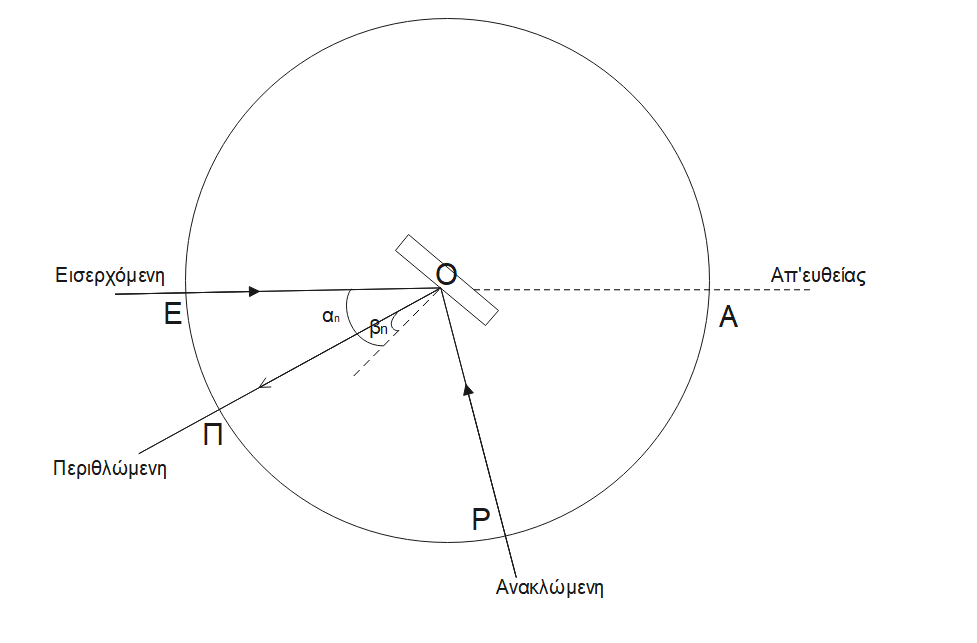
\includegraphics[width=0.6\linewidth]{2nd.png}
		\caption{ }
		\label{Im2}
	\end{figure}
	
Για το οπτικό φράγμα μας ισχύει η εξίσωση 	
	\begin{align}\label{6}
		d(sin\alpha_n+ sin\beta_n)=n\lambda 
	\end{align}
	όπου $d=1/N$ η σταθερά του φράγματος, n η τάξη του κροσσού συμβολής και $\lambda$ το μήκος κύματος της προσπίπτουσας δέσμης.
	\subsection*{Πειραματική Διάταξη}
	Η πειραματική διάταξη αποτελείται από: 
	\begin{itemize}
		\item[.] Λυχνία ατμών Νατρίου 
		\item[.] Τροφοδοτικό λυχνίας 
		\item[.] Κατευθυντήρα για την προσπίπτουσα δέσμη 
		\item[.] Γωνιόμετρο με βερνιέρο
		\item[.] Τηλεσκόπιο
		\item[.] Οπτικό φράγμα ανάκλασης ($Ν=1800mm^{-1})$
	\end{itemize}
	
	Η διάταξη φαίνεται στην παρακάτω Εικόνα (\ref{Im1}).
	\begin{figure}[h!]
		\centering
		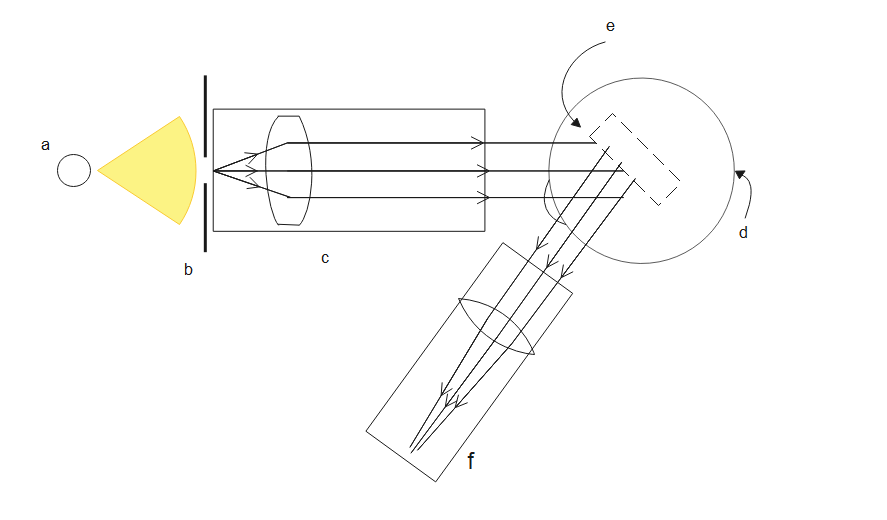
\includegraphics[width=0.8\linewidth]{setup.png}
		\caption{  a)Λάμπα Νατρίου, b) Λεπτή σχισμή, c) Κατευθυντήρας, d) Οπτική τράπεζα που περιστρέφεται. Στην βάση της υπάρχει ο γωνιομετρικός κύκλος, e) Οπτικό Φράγμα, f) τηλεσκόπιο}
		\label{Im1}
	\end{figure}
	
\subsection*{Πειραματική Διαδικασία - Επεξεργασία Μετρήσεων}	
	
	\subsubsection*{Μήκη κύματος φασματικών γραμμών}
	Αφού τοποθετήσουμε το φράγμα και θέσουμε σε λειτουργία την λυχνία, παρατηρούμε το φάσμα του νατρίου ποιοτικά (κόκκινο, κίτρινο, κίτρινο-πράσινο, πράσινο) από την περιθλώμενη δέσμη. Αρχικά καταγράφουμε την ένδειξη του γωνιομέτρου για την απ' ευθείας δέσμη και την ένδειξη για την ανακλώμενη δέσμη της λάμπας. 'Επειτα καταγράφουμε τις ενδείξεις για τις περιθλώμενες δέσμες. Τα αποτελέσματα φαίνονται στον Πίνακα (\ref{mat1})
	
	\begin{table}[h!]
		\centering
		\begin{tabular}{r|r}
			Σημείο Μέτρησης & $\theta(\pm0.1^o)$ \\\hline\hline
			A         & 170.3 \\ 
			P         & 230.0 \\ 
			$Π_{κοκ}$ & 305.9 \\ 
			$Π_{πρα}$ & 299.3 \\
			$Π_{κιτ}$ & 301.4 \\
		\end{tabular}
		\caption{Α: Απ'ευθείας, P:Ανακλώμενη,\\ $Π_{κοκ}$: Περιθλώμενη Κόκκινη, $Π_{πρα}$: Περιθλώμενη Πράσινη,\\ 	 $Π_{κιτ}$: Περιθλώμενη Κίτρινη }
		\label{mat1}
	\end{table}
	
	Για να χρησιμοποιήσουμε την σχέση (\ref{6}) και να βρούμε τα μήκη κύματος που αντιστοιχούν στην κάθε γωνία, θα πρέπει να ξέρουμε σε ποιό σημείο βρίσκεται η κάθετος στο φράγμα προκειμένου να βρούμε τις γωνίες ανάκλασης και περίθλασης. Από τον Πίνακα (\ref{mat1}) μπορούμε αρχικά να βρούμε την ένδειξη στο σημείο Ε που θα είναι $\alpha_E=(\underbrace{350.3}_{170.3+180.0}\pm0.1)^o$ και έπειτα την συνολική γωνία $E\hat{O}P$ που σχηματίζει η εισερχόμενη με την ανακλώμενη δέσμη, να την διαιρέσουμε δια δύο και να βρούμε την γωνία πρόσπτωσης $a_1$: 
	\begin{align*}
		\alpha_1 = 0.5( |230.0-350.3| \pm 0.1)^o \Rightarrow \boxed{\alpha_1 = (60.2\pm 0.1)^o}
	\end{align*}
	
Τώρα μπορούμε να βρούμε την θέση της καθέτου στο φράγμα:
	\begin{align*}
		n = ((\alpha_E+\alpha_1) \pm\delta n)^o \Rightarrow \boxed{n = (290.1\pm0.1)^o}
	\end{align*}

Εν τέλει είμαστε σε θέση να προσδιορίσουμε την γωνία περίθλασης για κάθε μήκος κύματος από την σχέση $\beta_{1,i}=|\Pi_{i} - n|$ και πλέον έχουμε όλες τις γωνίες ώστε να χρησιμοποιήσουμε την σχέση (\ref{6}). Άρα προκύπτει ο παρακάτω Πίνακας (\ref{mat2}): 
	\begin{table}[h!]
		\centering
		\begin{tabular}{r|r|r}
			Χρώμα & $\beta_{1,i}(\pm0.1^o)$ & $\lambda_{i}(nm)$\footnotemark \\\hline\hline 
			Πράσινο & 9.2  & $571\pm1$ \\ 
			Κίτρινο & 11.3 & $591\pm1$ \\ 
			Κόκκινο & 15.8 & $633\pm1$
		\end{tabular}
		\caption{i=κοκ,πρα,κιτ}
		\label{mat2}
	\end{table}
	\footnotetext{Το σφάλμα για κάθε μήκος κύματος προκύπτει από διάδοση $\delta\lambda_i=\sqrt{(\pdv{\lambda}{\alpha}\delta\alpha)^2+(\pdv{\lambda}{\beta_{1,i}}\delta\beta_{1,i})^2} = \sqrt{(d cos(\alpha)\delta\alpha)^2 + (dcos(\beta_{1,i})\delta\beta_{1,i})^2}=d\delta\alpha\sqrt{cos(a)^2 + cos(\beta_{1,i})^2}$}
	
	\subsubsection*{Ενεργειακή Διαφορά Κίτρινης γραμμής}
	
		Τώρα θα υπολογίσουμε την ενεργειακή διαφορά και που προκαλλεί η σύζευξη LS για την κίτρινη γραμμή από τον διαχωρισμό της σε δύο επιμέρους γραμμές. Επειδή το γωνιόμετρο που διαθέτουμε δεν έχει τόσο μεγάλη ακρίβεια ώστε να μπρούμε να μετρήσουμε απ' ευθείας την διαφορά στις γωνίες περίθλασης των δύο κίτρινων γραμμών θα κάνουμε ένα τρικ. 
		Συγκεκριμένα, εφ΄ όσον η διαφορά είναι ορατή μεσω του τηλεσκοπίου, παίρνουμε δύο μετρήσεις στρίβωντας το γωνιόμετρο δύο φορές την μεταξύ τους απόσταση προς τα δεξιά της μίας γραμμής και προς τα αριστερά της άλλης. Αυτή η στροφή προφανώς δεν μπορεί να είναι ακριβής και πραγματοποιείται ''με το μάτι'' και αυτό είναι το σημείο όπου εισέρχεται μεγάλο σφάλμα (το θεωρώ $0.2^o$). 
		
		Έχουμε από πριν ότι η γωνία περίθλασης του κίτρινου είναι στην θέση $301.4^o$ ενώ από την παραπάνω διαδικασία μετρήσαμε την μία γωνία στις $301.2^o$, ενώ την άλλη στις $301.6^o$, επομένως η διαφορά είναι $\Delta\beta_{1,κιτ} = 0.4/5 = 0.08^o$, άρα 
		
		\begin{align*}
			\Delta\beta_{1,κιτ} = ( 0.08 \pm 0.04 ) ^o
		\end{align*}
	
	Ωστόσο, εμείς σε τελική ανάλυση θέλουμε να υπολογίσουμε την ενεργειακή διαφορά που επιφέρει η σύζευξη LS, η οποία δίνεται από την σχέση: 
		\begin{align*}\label{7}
			\Delta E = h \Delta f = hc\Delta(\frac{1}{\lambda}) = hc\left(\frac{1}{\lambda_{left}}-\frac{1}{\lambda_{right}}\right)\numberthis
		\end{align*}
		
Άρα αν θεωρήσουμε ότι η μέτρηση για το κίτρινο $\beta_{1,κιτ} = (11.3\pm0.1)^o$ ήταν περίπου στο μέσο των δύο γραμμών, τότε έχουμε για την αριστερή και την δεξιά αντίστοιχα ότι $\beta_{1,κιτ,left} = (11.26 \pm 0.20)^o$, $\beta_{1,κιτ,right} = ( 11.34 \pm 0.20)^o$. Από την σχέση (\ref{6}) προκύπτουν τα δύο μήκη κύματος $\lambda_{left} = (590.6 \pm 2.1)nm $ και $\lambda_{right} = (591.3 \pm 2.1)nm $. 		
		
		
		%Άρα με τα δεδομένα που έχω θα πρέπει να υπολογίσω την διαφορά εντός της παρένθεσης. Από την σχέση (\ref{6}) και δεδομένου ότι οι γωνίες $\beta_{1,i}$ είναι μικρές, δηλαδή $sin\beta_{1,i} \simeq \beta_{1,i}$, παίρνω: 
%		\begin{align*}
%		  \left\{ d \right.
%		\end{align*}

%Άρα από την σχέση (\ref{6}) προκύπτει η παρακάτω διαφορά στις ενέργειες\footnotemark 
%	 \begin{align*}
%	 	\Delta E = (2.7 \pm )\times10^{-3}eV
%	 \end{align*}
%
%\footnotetext{Από διάδοση έχουμε $\delta\Delta E = \sqrt{\left( \pdv{\Delta E}{\lambda_{left}}\delta\lambda_{left} \right)^2+\left( \pdv{\Delta E}{\lambda_{right}}\delta\lambda_{right} \right)^2} = hc\delta\lambda_{left} \sqrt{\frac{1}{\lambda_{left}^4}+\frac{1}{\lambda_{right}^4}}$}

Άρα από την σχέση (\ref{7}) προκύπτει διαφορά στις ενέργειες $\Delta E = 2.7\times10^{-3}eV$. Η απόκλιση από το θεωρητικά αναμενόμενο ($2.1\times10^{-3} eV)$ είναι $0.6\times10^{-3}eV$, δηλαδή της τάξης του $\sim30\%$.

\subsection*{Περί Ανώτερων Τάξεων}

	Αν χρησιμοποιήσουμε το ίδιο οπτικό φράγμα, τότε από την σχέση (\ref{6}), για περίθλαση δεύτερης τάξης, $n=2$ και για το κίτρινο μήκος κύματος $\lambda_{κιτ} = (591\pm1)nm$ παίρνω ότι 
	\begin{align*}
		sin\alpha + sin\beta_2 \simeq 2.13
	\end{align*}
 
 το οποίο είναι άτοπο, άρα με το εν λόγω φράγμα δεν μπορούμε να παρατηρήσουμε καν περίθλαση δεύτερης και προφανώς ούτε ανώτερης τάξης για το κίτρινο μήκος κύματος.
 
% Αν θέλουμε να παρατηρήσουμε περίθλαση ανώτερης τάξης, τότε πάλι από την σχέση (\ref{6}) παίρνουμε:
% 	\begin{align*}
% 		\beta_n = arcsin(\frac{n\lambda}{d} - sin\alpha)
% 	\end{align*}
% 	και για να έχει νοήμα η παραπάνω σχέση θα πρέπει να ισχύει: 
% 	\begin{align*}
% 		0\leq& \frac{n\lambda}{d} - sin\alpha\leq1 \xRightarrow{N=1/d} \\ 
% 		%
% 		%
% 		%\underbrace{\frac{sin\alpha-1}{n\lambda} \leq}_{\alpha\in(0,90)\rightarrow\text{ισχύει πάντα}}& \frac{1}{d}\leq\frac{1 + sin\alpha}{n\lambda}\xRightarrow \\ 		
% 		%d\geq &\frac{n\lambda}{1+sin\alpha}\xRightarrow{\alpha=(60.2\pm0.1)^o } \\ 
% 		%d\geq &0.535\cdot n \lambda\\
% 		%N \leq &\frac{1+sin\alpha}{n\lambda} 	
% 		%
% 		%
% 		\frac{sin\alpha}{n\lambda}\leq& N \leq \frac{1+sina}{n\lambda}  \\
% 	\end{align*}
% 	
% 	Άρα π.χ. για $n=2$ και για το κίτρινο χρώμα, θα πρέπει να έχουμε από





%	Αν θέλουμε να παρατηροήσουμε περίθλαση ανώτερης τάξης, τότε έχουμε ότι $\lambda_{min}= 570.9nm$ και $\lambda_{max}=633.4 nm$, άρα από την (\ref{6}): 
%		\begin{align*}
%			\lambda_{min}\leq& \lambda \leq\lambda_{min} \Rightarrow \\
%			\lambda_{min}\leq& \frac{d(\cancelto{0.8678}{sin\alpha}+\sin\beta)}{n} \leq\lambda_{min} \Rightarrow \\
%			\lambda_{min}\leq& \lambda \leq\lambda_{min} \Rightarrow \\
%		\end{align*}

\subsection*{Συμπεράσμα}
	Συμπερασματικά, τα αποτελέσματα είναι ικανοποιητικά, στα πλαίσια των αναμενόμενων αποκλίσεων, πέρα από τους υπολογισμούς για τον διαχωρισμό που είχε απόκλιση $\sim 30\% $ και όπου κάναμε το πειραματικό τρικ για να αυξήσουμε κατά μία έννοια την ακρίβεια του οργάνου μας
\end{document}